\documentclass[]{article}

%% Reproducible builds
\pdfinfoomitdate=1
\pdftrailerid{}
\pdfsuppressptexinfo=-1

\usepackage[margin=0.9in]{geometry}

\usepackage{enumitem}
\usepackage{graphicx}
\usepackage{hyperref}
\usepackage{float}
\usepackage{listings}
\lstset{
	language=bash,
	basicstyle=\ttfamily
}

\graphicspath{{images/testing-policy/}}

\hypersetup{
	colorlinks=true,
	linkcolor=blue,
	filecolor=magenta,
	urlcolor=cyan,
}

%opening
\title{Testing Policy - Docks}
\author{TripleParity}
\date{}

\begin{document}
\maketitle

\tableofcontents

\section{Testing Process}

\subsection{Peer Review}
Before code can be merged into the develop branch a Pull Request has to be created.
Three reviews are required from other developers before the pull request
can be merged into develop.

During peer reviews the following should be checked:
\begin{itemize}
	\item Architectural problems - will this cause problems in the future?
	\item Compliance with requirements and design - is that what we need?
	\item Coding Standards - proper code formatting and security standards?
\end{itemize}

\begin{figure}[H]
	\centering
	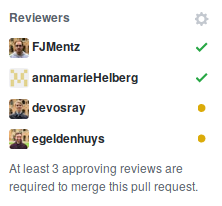
\includegraphics[scale=0.5]{github_3_reviews_required.png}
	\caption{At least 3 peer reviews are needed for a feature to be merged}
\end{figure}

\begin{figure}[H]
	\centering
	
\includegraphics[scale=0.5]{github_approved_review.png}
	\caption{An example of a positive peer review}
\end{figure}

\subsection{Automated Testing and Continuous Integration}
When a commit is made to the 'docks-ui' repository on GitHub two
processes are started:
\begin{itemize}
	\item \href{https://travis-ci.org/TripleParity/docks-ui/branches}{Travis CI} Builds the repository
	\item \href{https://hub.docker.com/r/tripleparity/docks-ui/builds/}{Docker Hub} builds the repository and creates a Docker Image that can be deployed in production
\end{itemize}

\subsubsection{Travis CI}
The history of test reports for Travis CI can be viewed at \url{https://travis-ci.org/TripleParity/docks-ui/branches}.
If the build was not successful it will be marked as 'failed' \\
\\
Travis CI is used for running tests associated with each repository. \\
\\
For the frontend Angular generates a set of tests for each component to verify
that the component was successfully created. These tests run inside a
headless (no screen required) Chrome browser.

The backend also has a suite of unit tests that are executed on Travis CI.

\begin{figure}[H]
	\centering
	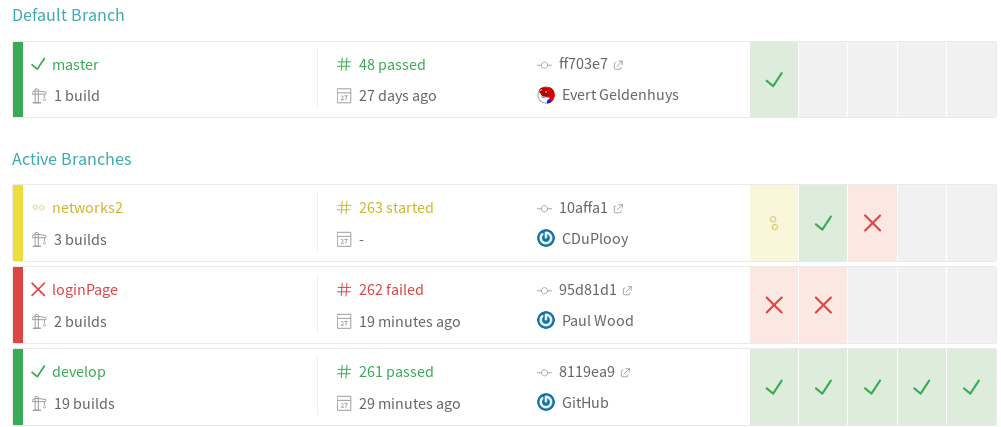
\includegraphics[scale=0.5]{travis_build_history.png}
	\caption{Screenshot of Travis CI branch build history}
\end{figure}

\begin{figure}[H]
	\centering
	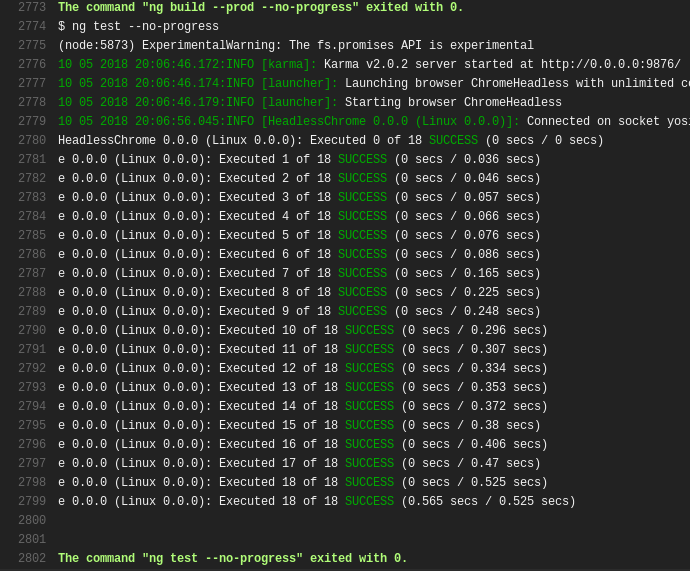
\includegraphics[scale=0.5]{travis_ui_tests_output_1.png}
	\caption{18 UI tests running on Travis}
\end{figure}

\subsubsection{Docker Cloud}
Docker images are build on \href{https://cloud.docker.com/}{Docker Cloud}.
These image can then be deployed in a production environment or for development and testing.
Images can be viewed at \url{https://hub.docker.com/u/tripleparity/}

\begin{figure}[H]
	\centering
	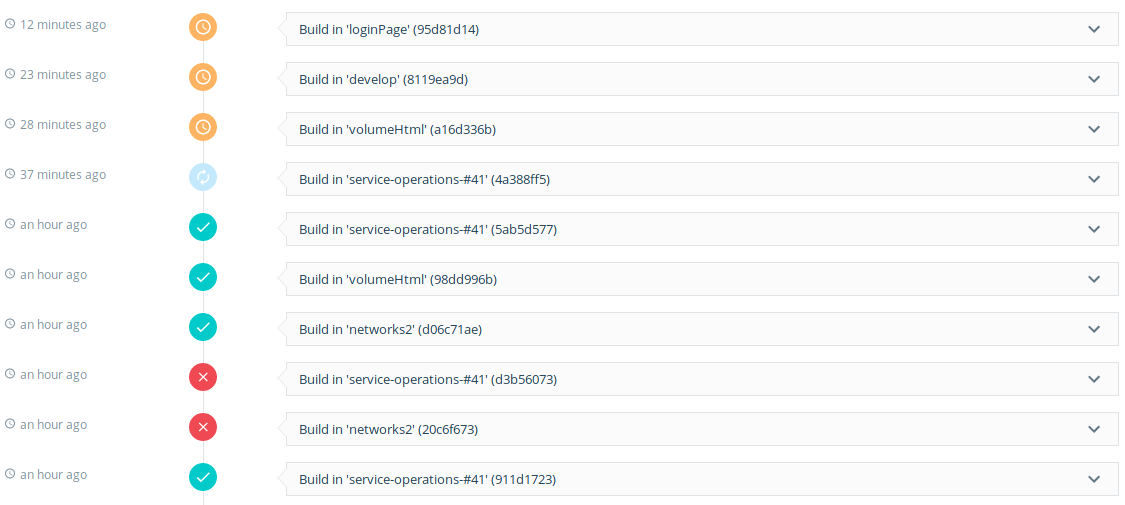
\includegraphics[scale=0.5]{docker_cloud_build_history.png}
	\caption{Screenshot of Docker Cloud Build History}
\end{figure}

\end{document}
